\documentclass[12pt]{amsart}
\usepackage[left=.5in,top=.5in,right=.5in,bottom=.5in]{geometry}                % See geometry.pdf to learn the layout options. There are lots.
\geometry{letterpaper}                   % ... or a4paper or a5paper or ... 
%\geometry{landscape}                % Activate for for rotated page geometry
%\usepackage[parfill]{parskip}    % Activate to begin paragraphs with an empty line rather than an indent
\usepackage{graphicx}
\usepackage{amssymb}
\usepackage{epstopdf}
\usepackage{float}
\usepackage{multicol}
\usepackage{cite}
\DeclareGraphicsRule{.tif}{png}{.png}{`convert #1 `dirname #1`/`basename #1 .tif`.png}
\setlength{\parskip}{0pt}
\setlength{\parindent}{0.5cm}
\usepackage{times}
\usepackage{wrapfig}
\usepackage{hyperref}
\newenvironment{Figure}
  {\par\medskip\noindent\minipage{\linewidth}}
  {\endminipage\par\medskip}
\usepackage[small]{caption}
\pagenumbering{gobble}
\usepackage[small,compact]{titlesec}


\begin{document}

\begin{flushleft}
{\Large
Low-dimensional structure of neural correlations in cortical microcircuits
}
\\
\vspace{6pt}
Dimitri Yatsenko, 
Kre\v{s}imir Josi\'{c},
Alexander S.~Ecker,
Emmanouil Froudarakis,
R.~James Cotton,
Andreas S.~Tolias
\end{flushleft}
\subsection*{Summary}
Ambitious projects currently under way aim to record the activity of ever larger and denser subsets of neurons in behaving animals.  It is commonly anticipated that correlations measured in such recordings will uncover aspects of functional organization of neural circuits.  However, estimation and interpretation of large correlation matrices from finite recordings can be challenging.  Estimation can be improved by regularization: the biasing of the estimate toward a low-dimensional, less variable approximation.  The amount of improvement depends on how closely the reduced approximation captures the dominant interactions with fewest terms. Therefore, the selection of the most efficient estimator is an empirical question dependent on the system under investigation. 

We compared regularized correlation matrix estimators biased toward four respective families of low-dimensional correlation structures: independent, latent factors, sparse partial correlations, and sparse partial correlations + latent factors.  The estimators' performance was evaluated on the noise correlation matrices from spatially compact groups of 91--314 neurons (average 206) in mouse visual cortex (31 sites in 24 animals) acquired by \emph{in vivo} fast 3D random-access two-photon imaging of calcium signals. Recordings lasting between 15 and 20 minutes were deconvolved and binned at 150 ms. Each estimator was optimized and evaluated by nested cross-validation.  We found that both sparse partial correlations and latent factors were required for efficient estimation.  In addition to reducing estimation error, optimized estimates provided compact representations of the correlation structure decomposed into a sparse network of pairwise interactions and global diffuse fluctuations. The density of positive interactions in these networks decreased rapidly with distance and with difference in orientation preference, whereas negative interactions were less selective. In ongoing studies, we seek to relate these elements of the correlation structure to circuits' anatomical organization, stimulus conditions, and brain states.

\subsection*{Additional Details}
\subsubsection*{Central Questions} We pursued two related aims: (a) improved estimation of correlation matrices and (b)~discovery of low-dimensional structure of correlations in recordings of multineuronal activity. 

\subsubsection*{Approach}
\begin{wrapfigure}[16]{r}{0.4\textwidth}
\centering
\vspace{-6pt}
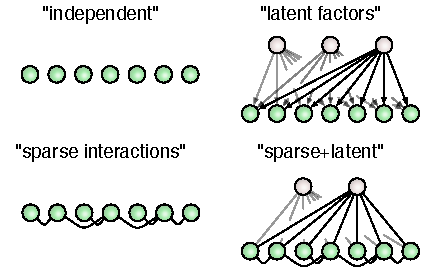
\includegraphics{./Simulation.pdf}
\caption{Families of low-dimensional correlation target estimates for regularization. Recorded neurons are in green whereas inferred latent factors are light-colored. Edges denote linear associations (non-zero partial correlations).}

\label{fig:graphical}
\end{wrapfigure}
Both aims benefit from \emph{regularization}: the deliberate biasing (`shrinkage') of the usual sample correlation matrix toward a low-dimensional \emph{target estimate}. 

We constructed for covariance estimators based on four low-dimensional target estimates of covariance matrices  (\autoref{fig:graphical}): 
The target of the first estimator has a diagonal covariance matrix, which describes a population of independent neurons \cite{Ledoit:2004}. 
The target of the second estimator is a multifactor model \cite{Fan:2008}, which describes a population of neurons driven together by a small number of latent factors with negligible direct interactions.
The third estimator is based on the assumption that all correlations are the result of direct linear interactions between a fraction of observed cell pairs. This assumption is enforced by reducing to zero the majority of coefficients of the inverse of the correlation matrix \cite{Dempster:1972}. 
Finally, the fourth estimator allows for both common latent units and sparse local interactions between recorded neurons.  
In this estimator, the correlation matrix is modeled as the inverse of a sum of a sparse and a low-rank component \cite{Chandrasekaran:2010}.

\subsubsection*{Results}
Each estimator was optimized and evaluated with respect to cross-validated multivariate Gaussian log-likelihood.  First, with synthetic data, we demonstrated that estimators whose regularization targets matched the true correlation structure outperformed other estimators (data to be presented).  

We then estimated the correlation matrices of population calcium signals of large groups of cells (91--314 neurons, averarge 206 in 31 sites from 24 animals) in small volumes of visual cortex during visual stimulation \cite{Cotton:2013}. We found that the sparse+latent estimator consistently outperformed all other estimators (data to be presented).

In addition to minimizing the estimation error, the sparse+latent estimator revealed sparse networks of linear interactions such as shown in \autoref{fig:reconstruction} and several shared latent units (not shown).
Individual imaged sites varied greatly in the number of significant latent units and the sparsity of direct interations (data to be presented).
We analyzed how the distribution of these interactions compared to the distribution of the usual sample correlations as a function of the difference in preferred orientation, vertical distance, and lateral distance in the cortex \autoref{fig:summary}. The patterns of inferred interactions differed substantially from patterns of most significant correlations (data to be presented).
\begin{multicols}{2}
\begin{Figure}
  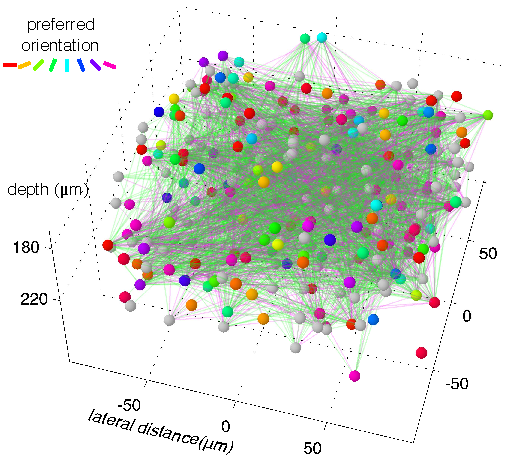
\includegraphics{./Reconstruction.pdf}
  \captionof{figure}{An example of 3D arrangement of recorded cells with color-coded orientation preference and edges indicating the network of positive (green) and negative interactions (magenta) as revealed by the sparse+latent estimator. The latent units are not shown.}
  \label{fig:reconstruction}
\end{Figure}

\begin{Figure}
  \centering
  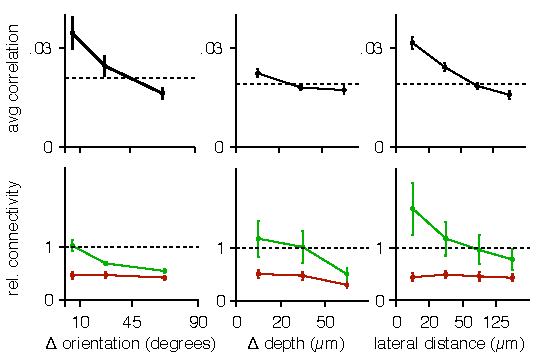
\includegraphics{./Summary.pdf}
  \captionof{figure}{Top row: average sample correlations across all sites. Bottom row: normalized interaction probabilities of the sparse+latent estimator with positive interactions shown in green and negative interactions show in red. Left column: as a function of difference in preferred orientation. Middle column: as a function of difference in cortical depth at small lateral distances. Right column: as a function of lateral distance at the same cortical depth. Dottted lines indicate averages across all conditions across all sites included in each analysis.}
  \label{fig:summary}
\end{Figure}
\end{multicols}

\subsubsection*{Significance}
In this empirical study, we identified the most efficient of several estimators of correlation matrices of activity fluctuations in cortical microcircuits. The resulting estimates effectively decomposed the correlation structure into direct interactions between pairs of neurons and common diffuse fluctuations. The physiological interpretation of these components remains in question and must be addressed by additional experiements where synaptic connectivity, cell types, and local field potentials may be used to corroborate such interpretations. 


\bibliographystyle{plos2009}
\bibliography{references.bib}

\end{document}  
